\documentclass{article}

\usepackage{graphicx}
\usepackage{tikz}
\usepackage{tikzsymbols}
\usetikzlibrary{calc,patterns,shapes.geometric}
\pagestyle{empty}
\usepackage[margin=0pt]{geometry}
\geometry{papersize={14in,12in}}

\def\centerarc[#1](#2)(#3:#4:#5){\draw[#1] ($(#2)+({#5*cos(#3)},{#5*sin(#3)})$) arc (#3:#4:#5);}

\begin{document}
	\begin{figure}
		\centering
		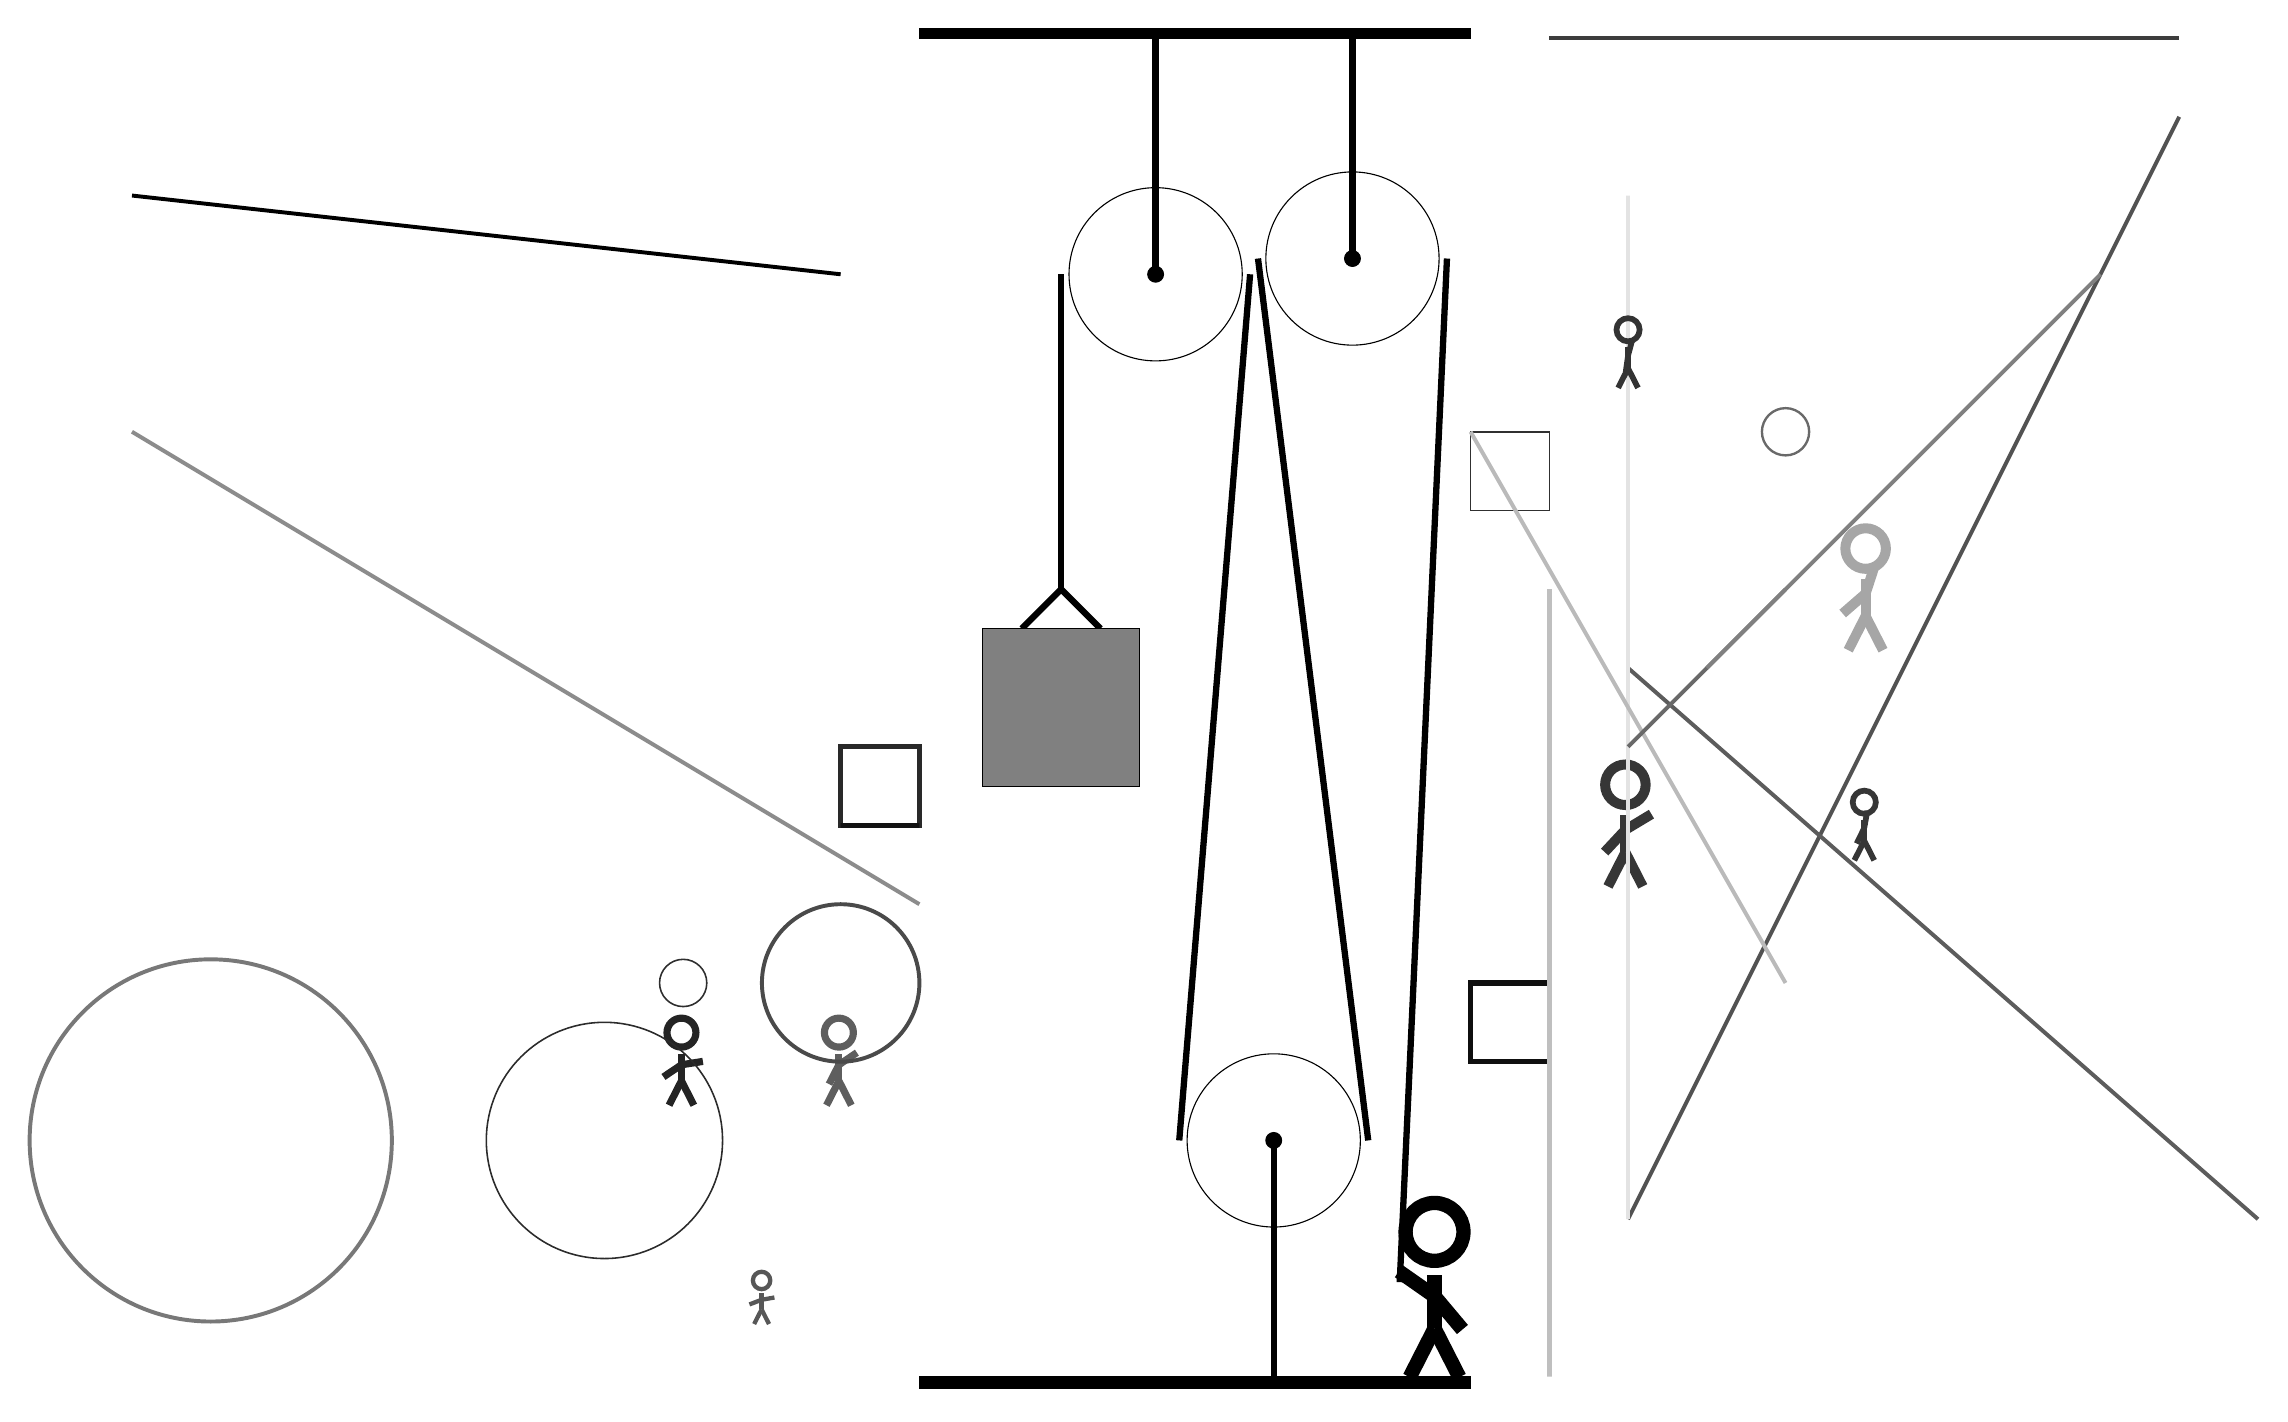
\begin{tikzpicture}
			%%%%% START %%%%%
			
			\draw[fill=black] (-2, 14) rectangle (5, 14.125);
			
			\draw (1, 11) circle (1.1);
			\draw[fill=black] (1, 11) circle (0.1);
			\draw[line width=0.8mm]  (1, 14) -- (1, 11);
			
			\draw[fill=white](2.5, 0) circle (1.1);
			\draw[fill=black] (2.5, 0) circle (0.1);
			\draw[line width=0.8mm]  (2.5, -3) -- (2.5, 0);
			
			\draw[line width=0.7mm, color=black!94] (6, 1) rectangle (5, 2);
			
			\draw[line width=0.5mm, color=black!68](7, -1) -- (14, 13);
			\draw[line width=0.7mm, color=black!84] (-3, 5) rectangle (-2, 4);
			\draw[line width=0.5mm, color=black!45](-2, 3) -- (-12, 9);
			\draw [line width=0.3mm, color=black!59](9, 9) circle (0.3);
			\node[line width=0.2mm, color=black!79] at (7, 4) {\Strichmaxerl[7][47][31]};
			
			\node[line width=0.3mm, color=black!79] at (10, 4) {\Strichmaxerl[4][64][80]};
			
			\draw[line width=0.7mm, color=black!25] (6, 7) rectangle (6, -3);
			\node[line width=0.5mm, color=black!86] at (-5, 1) {\Strichmaxerl[5][34][9]};
			\draw[line width=0.5mm, color=black!64](7, 6) -- (15, -1);
			\draw[line width=0.2mm, color=black!81] (5, 9) rectangle (6, 8);
			\draw[line width=0.6mm, color=black!11] (7, -1) rectangle (7, 12);
			\draw[line width=0.5mm, color=black!100](-3, 11) -- (-12, 12);
			
			\node[line width=0.7mm, color=black!66] at (-4, -2) {\Strichmaxerl[3][21][10]};
			\draw[line width=0.5mm, color=black!27](9, 2) -- (5, 9);
			\draw[line width=0.5mm, color=black!59](9, 7) -- (7, 5);
			\node[line width=0.5mm, color=black!63] at (-3, 1) {\Strichmaxerl[5][63][34]};
			\draw[line width=0.7mm, color=black!93] (-2, 4) rectangle (-3, 4);
			\draw[line width=0.5mm, color=black!50](8, 6) -- (13, 11);
			\draw [line width=0.5mm, color=black!53](-11, 0) circle (2.3);
			\draw [line width=0.2mm, color=black!82](-5, 2) circle (0.3);
			
			\draw[line width=0.5mm, color=black!76](6, 14) -- (14, 14);
			\draw [line width=0.2mm, color=black!83](-6, 0) circle (1.5);
			\draw [line width=0.5mm, color=black!71](-3, 2) circle (1.0);
			\node[line width=0.5mm, color=black!35] at (10, 7) {\Strichmaxerl[7][41][72]};
			
			\node[line width=0.6mm, color=black!80] at (7, 10) {\Strichmaxerl[4][82][75]};
			
			
			\draw[fill=white](3.5, 11.2) circle (1.1);
			\draw[fill=black] (3.5, 11.2) circle (0.1);
			\draw[line width=0.8mm] (3.5, 14) -- (3.5, 11.2);
			
			\draw[line width=0.8mm] (-0.7, 6.5) -- (-0.2, 7.0) -- (0.3, 6.5);
			\draw[fill=black!50] (-1.2, 6.5) rectangle (0.8, 4.5);
			
			\draw[line width=0.8mm] (-0.2, 11) -- (-0.2, 7.0);
			\centerarc[line width=0.8mm](1, 11)(0:180:1.2000000000000002);
			\draw[line width=0.8mm](2.2, 11) -- (1.3, 0);
			\centerarc[line width=0.8mm](2.5, 0)(180:360:1.2000000000000002);
			\draw[line width=0.8mm](3.7, 0) -- (2.3, 11.2);
			\centerarc[line width=0.8mm](3.5, 11.2)(0:180:1.2000000000000002);
			\draw[line width=0.8mm](4.7, 11.2) -- (4.1, -1.8);
			
			\node at (4.5, -1.9) {\Strichmaxerl[10][-35][-50]};
			
			\draw[fill=black] (-2, -3) rectangle (5, -3.15);
			
			%%%%% END %%%%%
		\end{tikzpicture}
	\end{figure}	
\end{document}